\documentclass[12pt, a4paper, twoside]{article}
\usepackage{../labreport}
\usepackage{pdfpages}
\usepackage{circuitikz}
\usepackage{adjustbox}

\setlabreportopts[authors={Nandor Kovacs \& Céline Schuster},
    title={Glühlämpchen},
    subtitle={Aufbau von einfachen Schaltkreisen, und die Messung von Strom und Spannung},
    date={\today},
    labdate={24. März 2022}
]

\pgfplotsset{compat=1.16}
\begin{document}
\maketitlepage
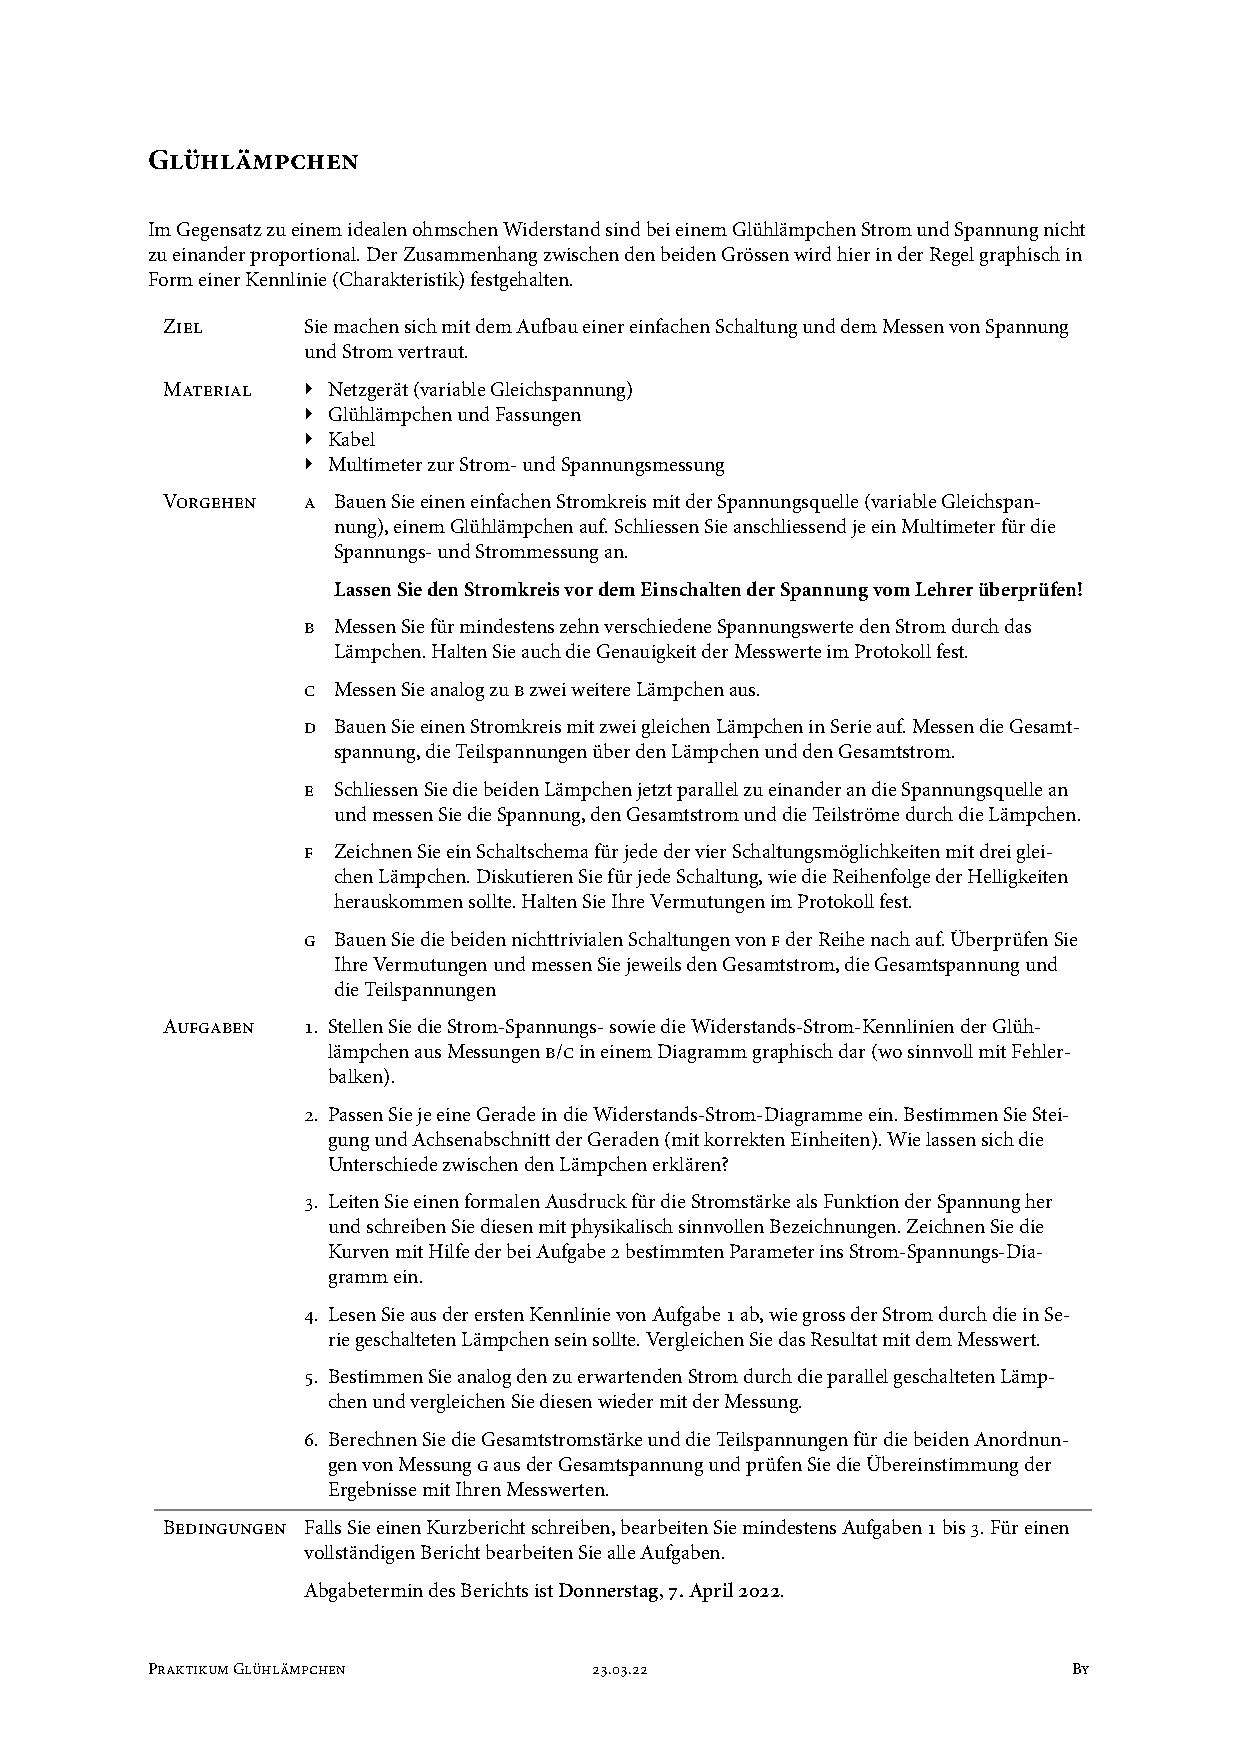
\includepdf[pages={1}]{aufgabenstellung.pdf}
\section{Einleitung}
Im Gegensatz zu herkömmlichen Widerständen (R) sind Strom (I) und Spannung (U) bei Glühlampen nicht proportional zueinander. Dennoch stehen diese Grössen in einem gewissen Verhältnis zueinander. Ziel dieses Berichts ist es, das Verhalten einer Glühbirne zu analysieren. Zunächst werden die Auswirkungen auf das Verhältnis zwischen Spannung und Stromstärke untersucht in den Parallel- und Serieschaltung von Glühbirnen und die Spannungsverteilung bei drei nicht trivialen Schaltungen.


\section{Theorie}
Der Widerstand $R$ ist gleich zur Stromspannung über der Stromstärke.
\begin{align*}
  R = \frac{V}{A}
\end{align*}

Für herkömmliche Widerstände gilt:

\begin{align*}
  R_{serie}              & = \sum_{i}R_i            \\
  \frac{1}{R_{parallel}} & = \sum_{i} \frac{1}{R_i}
\end{align*}
\cite{FoTa, S.176}
\\
\\
Glühlampen haben 2 wichtige Parameter was Stromkreise angeht:
\begin{list}{-}{}
  \item Den Kaltwiderstand, das ist der Widerstand $R_{kalt}$, der herrscht wenn kein Strom fliesst.
  \item Der warmwiderstands Koeffizient $r$. Der Warmwiderstand $R_{warm}$ ist $r * I$.
\end{list}
\section{Experiment}
Das folgende Experiment besteht aus verschiedenen Stromkreisen und deren Messungen. 
Für den folgenden Stromkreis haben wir zehn Messungen für Lampe 1, fünf für Lampe 2 und weitere fünf für Lampe 3. Für alle zehn werden unterschiedliche Spannungen angelegt, wie in den folgenden Grafiken dargestellt. \\
\\
Falls nichts anderes steht sind alle Werte für $U$ in Volt, und alle Werte für $A$ in Ampere angegeben.
\circuit{
  (0, 0) to[vsource] (0, 5) to[lamp] (8, 5) to[rmeterwa, t=A, l=$I_{gemessen}$] (8, 0) -- (0, 0)
  (2, 5) -- (2, 6) to[rmeterwa, t=V, l=$U_{gemessen}$] (6, 6) -- (6, 5)

}

\datatable{c|c|c}{\csvcoli & \csvcolii & \csvcoliii}{Lämpchen 1}{$U_{start}$ & $U_{gemessen}$ & $I_{gemessen}$}{a_lamp1.csv}{a_lamp1}
\datatable{c|c|c}{\csvcoli & \csvcolii & \csvcoliii}{Lämpchen 2}{$U_{start}$ & $U_{gemessen}$ & $I_{gemessen}$}{a_lamp2.csv}{a_lamp2}
\datatable{c|c|c}{\csvcoli & \csvcolii & \csvcoliii}{Lämpchen 3}{$U_{start}$ & $U_{gemessen}$ & $I_{gemessen}$}{a_lamp2.csv}{a_lamp3}

Für die nächsten beiden Stromkreise haben wir jeweils eine Messung, da wir uns im Folgenden nicht auf die spezifischen Werte, sondern auf die Position der Lampen konzentrieren:

\circuit{
  (0, 0) to[vsource] (0, 5) to[lamp, l=1] (4, 5) to[lamp, l=2] (8, 5) to[rmeterwa, t=A, l=$I_{total}$] (8, 0) -- (0, 0)
  (1, 5) -- (1, 6) to[rmeterwa, t=V, l=$U_{gemessen}$] (7, 6) -- (7, 5)
}

\datatable{c|c|c|c|c}{\csvcoli & \csvcolii & \csvcoliii & \csvcoliv & \csvcolv}{In Serie geschaltet}{$U_{start}$ & $U_{gemessen}$ & $I_{total}$ & $U_{1}$ & $U_{2}$}{b_lamp1.csv}{serie}

\circuit{
  (0, 0) to[vsource] (0, 5) to[lamp, l=2] (8, 5) to[rmeterwa, t=A, l=$I_{total}$] (8, 0) -- (0, 0)
  (2, 5) -- (2, 6.5) to[lamp, l=1] (6, 6.5) -- (6, 5)
  (2, 5) -- (2, 3.5) to[rmeterwa, t=V, l=$U_{gemessen}$] (6, 3.5) -- (6, 5)
}

\datatable{c|c|c|c|c}{\csvcoli & \csvcolii & \csvcoliii & \csvcoliv & \csvcolv}{Parallel geschaltet}{$U_{start}$ & $U_{gemessen}$ & $I_{total}$ & $I_{1}$ & $I_{2}$}{c_lamp1.csv}{parallel}

Vor der Durchführung der Messungen haben wir die Intensität jeder Lampe unter Berücksichtigung ihrer Position geschätzt. Es ist erwähnenswert, dass die Helligkeit der Lampen von der durch sie fließenden Spannung abhängt. 
Anschließend führen wir Messungen durch, um unsere Annahmen zu überprüfen.

\circuit{
  (0, 0) to[vsource] (0, 5)
  to[lamp, l=1] (8/3, 5) to[lamp, l=2] (16/3, 5) to[lamp, l=3]
  (8, 5) -- (8, 0) -- (0, 0)
}

Vermutung: 1, 2 und 3 alle gleich hell \\
Beobachtung: Unsere Vermutung war richtig

\datatable{c|c|c|c|c|c}{\csvcoli & \csvcolii & \csvcoliii & \csvcoliv & \csvcolv & \csvcolvi}{F$i$}{$U_{start}$ & $U_{gemessen}$ & $I_{total}$ & $U_{1}$ & $U_{2}$ & $U_{3}$}{f_1.csv}{f1}

\circuit{
  (0, 0) to[vsource] (0, 5)
  to[lamp, l=1] (4, 5) to[lamp, l=3]
  (8, 5) -- (8, 0) -- (0, 0)
  (1, 5) -- (1, 6) to[lamp, l=2] (7, 6) -- (7, 5)
}

\datatable{c|c|c|c|c|c|c}{\csvcoli & \csvcolii & \csvcoliii & \csvcoliv & \csvcolv & \csvcolvi & \csvcolvii}{F$ii$}{$U_{start}$ & $U_{gemessen}$ & $I_{total}$ & $U_{1}$ & $U_{2}$ & $U_{3}$ & $U_{1 + 3}$}{f_2.csv}{f2}

Vermutung: 1 und zwei sind gleich hell, 3 ist stärker wie 1 und 2\\
Beobachtung: Unsere Vermutung war richtig

\circuit{
  (0, 0) to[vsource] (0, 5)
  to[lamp, l=1] (3, 5) --
  (4, 5) -- (4, 6) to[lamp, l=2] (7, 6) -- (7, 5)
  (4, 5) -- (4, 4) to[lamp, l=3] (7, 4) -- (7, 5) --
  (8, 5) -- (8, 0) -- (0, 0)
}

\datatable{c|c|c|c|c|c|c}{\csvcoli & \csvcolii & \csvcoliii & \csvcoliv & \csvcolv & \csvcolvi & \csvcolvii}{F$iii$}{$U_{start}$ & $U_{gemessen}$ & $I_{total}$ & $U_{1}$ & $U_{2}$ & $U_{3}$ & $U_{2 + 3}$}{f_3.csv}{f3}

Vermutung: 1 ist am stärksten, 2 und 3 sind gleichstark.\\
Beobachtung: Unsere Vermutung war richtig


\circuit{
  (0, 0) to[vsource] (0, 5)
  to[lamp, l=2] (8, 5)
  (2, 5) -- (2, 6.5) to[lamp, l=1] (6, 6.5) -- (6, 5)
  (2, 5) -- (2, 3.5) to[lamp, l=3] (6, 3.5) -- (6, 5)
  (8, 5) -- (8, 0) -- (0, 0)
}

Hier haben wir keine Messungen gemacht \\

Vermutung: Alle sind gleichstark \\
Beobachtung: Unsere Vermutung war richtig

\section{Aufgaben}
\subsection{Strom-Spannungs- \& Wiederstands-Strom-Kennlinien}

\datadiagram{
  yticklabel style={
      /pgf/number format/fixed,
      /pgf/number format/precision=2},
  enlargelimits=0.2,
  ylabel={Stromstärke $I$ in Ampere},
  xlabel={Spannung $U$ in Volt}
}{
  \addplot+[color=red] table[x expr=\thisrow{v}, y expr=\thisrow{a}, col sep=comma] {a_lamp1.csv};
  \addplot+[color=green] table[x expr=\thisrow{v}, y expr=\thisrow{a}, col sep=comma] {a_lamp2.csv};
  \addplot+[color=cyan] table[x expr=\thisrow{v}, y expr=\thisrow{a}, col sep=comma] {a_lamp3.csv};
}

\datadiagram{
  xticklabel style={
      /pgf/number format/fixed,
      /pgf/number format/precision=2},
  enlargelimits=0.2,
  ylabel={Widerstand $R$ in Ohm},
  xlabel={Stromstärke $I$ in Ampere},
}{
  \addplot+[color=red] table[x expr=\thisrow{a}, y expr=\thisrow{v} / \thisrow{a}, col sep=comma] {a_lamp1.csv};
  \addplot+[color=green] table[x expr=\thisrow{a}, y expr=\thisrow{v} / \thisrow{a}, col sep=comma] {a_lamp2.csv};
  \addplot+[color=cyan] table[x expr=\thisrow{a}, y expr=\thisrow{v} / \thisrow{a}, col sep=comma] {a_lamp3.csv};
}

\subsection{Lineare regression an den Widerstands-Strom-Kennlinien}
\datadiagram{
  xticklabel style={
      /pgf/number format/fixed,
      /pgf/number format/precision=2},
  enlargelimits=0.2,
  ylabel={Widerstand $R$ in Ohm},
  xlabel={Stromstärke $I$ in Ampere},
}{
  \addplot+[color=red, clip mode=individual] table[x expr=\thisrow{a}, y expr=\thisrow{v} / \thisrow{a}, col sep=comma] {a_lamp1.csv};
  \addlegendentry{Lämpchen 1};
  \addplot+[color=lime, samples=4, domain=0.047:0.127]{1292.6*x + 44.6};
  \addlegendentry{1292.6*x + 44.6}
}
Lineare Regressionsfunktion:
$y = 1292.6\frac{V}{A^2}x + 44.6\frac{V}{A}$\\
Steigung: $1292.6\frac{V}{A^2}$\\
Achsenabschnitt: $44.6\frac{V}{A}$


\datadiagram{
  xticklabel style={
      /pgf/number format/fixed,
      /pgf/number format/precision=2},
  enlargelimits=0.2,
  ylabel={Widerstand $R$ in Ohm},
  xlabel={Stromstärke $I$ in Ampere},
}{
  \addplot+[color=green, clip mode=individual] table[x expr=\thisrow{a}, y expr=\thisrow{v} / \thisrow{a}, col sep=comma] {a_lamp2.csv};
  \addlegendentry{Lämpchen 2};
  \addplot+[color=lime, samples=4, domain=0.047:0.127]{1308.7*x + 37.7};
  \addlegendentry{1308.7*x + 37.7}
}
Lineare Regressionsfunktion: $y = 1308.7\frac{V}{A^2}x + 37.7\frac{V}{A}$\\
Steigung: $1308.7\frac{V}{A^2}$\\
Achsenabschnitt: $37.7\frac{V}{A}$

\datadiagram{
  xticklabel style={
      /pgf/number format/fixed,
      /pgf/number format/precision=2},
  enlargelimits=0.2,
  ylabel={Widerstand $R$ in Ohm},
  xlabel={Stromstärke $I$ in Ampere},
}{
  \addplot+[color=cyan, clip mode=individual] table[x expr=\thisrow{a}, y expr=\thisrow{v} / \thisrow{a}, col sep=comma] {a_lamp3.csv};
  \addlegendentry{Lämpchen 3};
  \addplot+[color=lime, samples=4, domain=0.047:0.127]{1417.6*x + 36.5};
  \addlegendentry{1417.6*x + 36.5}
}
Lineare Regressionsfunktion:
$y = 1417.6\frac{V}{A^2}x + 36.5\frac{V}{A}$\\
Steigung: $1417.6\frac{V}{A^2}$\\
Achsenabschnitt: $36.5\frac{V}{A}$
\\
\\
Der Achsenabschnitt wird durch den Kaltwiderstand der Glühlampe bestimmt.
Der Kaltwiderstand kann sich bei Glühlampen je nach Alter und Qualität von Lampe zu Lampe ändern.
\\
\\
Die Steigung beschreibt den Warmwiderstand der Glühlampe, proportional zur Stromstärke.
Diese wird durch die Eigenschaften des Glühdrahtes wie der Durchmesser und die Länge bestimmt.
Mit der Zeit können sich diese Eigenschaften ändern.
\\
Ab hier werden wir die Steigung $r$ nennen, und den Achsenabschnitt $R_{kalt}$.
\subsection{Stromstärke als Funktion der Spannung}
\begin{align*}
  R                      & = R_{warm} + R_{kalt}                             \\
  R_{warm}               & = r * I                                           \\
  \\
  I                      & = \frac{U}{R}                                     \\
  I                      & = \frac{U}{R_{warm} + R_{kalt}}                   \\
  I                      & = \frac{U}{r * I + R_{kalt}}                      \\
  I^2*r + I*R_{kalt} + U & = 0                                               \\
  I                      & = \frac{-R_{kalt}^2+\sqrt{R_{kalt}^2-4*r*U}}{2*U}
\end{align*}

\datadiagram{
  enlargelimits=0.2,
  ylabel={Stromstärke $I$ in Ampere},
  xlabel={Spannung $U$ in Volt}
}{
  \addplot+[color=red, samples=400, mark=none, domain=3:25]{((((44.8)^2)+sqrt(((44.6)^2)-(4*1292.6*-x)))/(2*x))};
  \addplot+[color=green,samples=400, mark=none, domain=3:25]{((((37.7)^2)+sqrt(((37.7)^2)-(4*1308.7*-x)))/(2*x))};
  \addplot+[color=cyan, samples=400, mark=none, domain=3:25]{((((36.5)^2)+sqrt(((36.5)^2)-(4*1417.6*-x)))/(2*x))};
}

\subsection{Messwerte der in Serie geschaltette Lampen mit der Kennlinie vergleichen}
In Tabelle \ref{table:serie} sehen wir unsere Messwerte für in Serie geschaltette Lampen.
Beide Lämpchen stehen unter einer Spannung von etwa 5 Volt, da bei der Serieschaltung sich die Spannung gleichmässig auf die Verbraucher oder Widerstände aufteilt falls der Widerstand gleich gross ist.
Bei 5 Volt erwarten wir aus dem Diagramm etwa eine Spannung von 0.05 Ampere.
Unsere Messung zeigt eine Spannung von 0.0496 Ampere.
Das ist nahe genug, denn das Ablesen von dem Diagramm ist ungenau genug um diesen Unterschied zu erlauben.

\subsection{Messwerte der Parallel geschaltette Lampen mit der Kennlinie vergleichen}
In Tabelle \ref{table:parallel} sehen wir unsere Messwerte für parallel geschaltette Lampen.
Wir haben eine Spannung von 10 Volt an den Stromkreis angehängt.
Beide Lämpchen stehen unter einer Spannung von etwa 10 Volt, da bei der Parallelschaltung beide Verbraucher oder Widerstände die volle Spannung erhalten.
Bei 10 Volt erwarten wir aus dem Diagramm eine Stromstärke von 0.075 Ampere.
Unsere Messungen zeigen eine Stromstärke von 0.0724 Ampere auf dem einen, und 0.0732 Ampere auf dem anderen Lämpchen.
Beide Messwerte sind wider weitaus im Fehlerbereich vom Ablesen aus dem Diagramm.

\subsection{Werte der nichttrivialen Stromkreise berechnen und mit den Messwerten vergleichen}
\subsubsection{$G_{ii}$}
Die Spannung die auf die zwei Wege fällt ist gleich.
Für beide Wege gilt, dass $I = U/R$. Da $R_2 = \frac{R_{1+3}}{2}$,
stimmt auch dass $I_2 = 2*I_{1+3}$.
Die Gesamtspannung beträgt 15 Volt, das heisst das $I_2 = 15V$, und $I_{1 + 3} = I_{1} = I{3} = 7.5V$.
Die Teilströme können wir also aus unserem Diagramm ablesen. Für 15 Volt erwarten wir etwa 0.09 Ampere, und für 7.5 Volt etwa 0.06 Ampere.
Daraus wissen wir, dass $U_2 = 0.09A$, und $U_1 = U_3 = 0.06A$. 
\\ 
\\
$U = U_1 + U_2 + U_3 = 0.21A$
\\
\\
Unsere Messung zeigt an, dass $U = 0.1535A$. Durch die ungenauigkeit der Ablesung aus dem Diagramm ist das innerhalb vom Fehlerbereich.
\subsubsection{$G_{iii}$}
$U_1 = U_{2+3}$, da durch $1$ sowie durch $(2 + 3)$ der volle Strom durchfliesst.
$R_1*2 = R_{2+3}$. $I = U * R$, deswegen $I_1 * 2 = I_{2 + 3}$.
Aus der Gesamtspannung von 15 Volt wissen wir deshalb, dass das Lämpchen 1 unter 10 Volt Spannung steht.
Da der volle Strom durch das Lämpchen 1 fliesst, langt es wenn wir den Wert für 10 Volt aus dem Diagramm lesen.
\\
\\
$U = 0.08$
\\
\\
Unsere Messung sagt, dass $U = 0.0817$, was sehr gut übereinstimmt.

\section{Fazit}
Der Widerstand von Glühlämpchen hängt von zwei wichtigen Parametern ab:
Ihr Kalt- und Warmwiderstand. Der Warmwiderstand ist proportional zur Stromstärke, ihr Kaltwiderstand ist aber konstant.
So erhalten wir eine Widerstands-Strom-Kennlinie, die die y-Achse nicht bei null schneidet, aber eine Gerade ist.
Die Steigung repräsentiert dabei einen Koeffizienten, der die Proportionalität zwischen der Stromstärke und des Widerstandes bestimmt.
\section{Reflektion}
Wir haben zuerst alle Werte für die Stromstärke in Milliampere eingetragen, haben dies aber erst sehr Spät bemerkt.
Hätten wir uns daran erinnert, oder hätten wir von Anfang an unsere Messungsdaten in SI Units eingetragen, hätten wir uns viel Mühe erspart.
In Zukunft werden wir eine Abmachung haben, dass, falls nichts anderes in der Excel Tabelle steht, alle werte in SI Units eingetragen sind.
\section{Anhang}
Versuchsanleitung und Originalprotokoll vom \labdate
\end{document}
